\documentclass{beamer}
\usetheme{Warsaw}
%\usepackage{caption}
%\DeclareCaptionType{copyrightbox}
\graphicspath{{../figures/}}
\usepackage{subcaption}
\captionsetup{compatibility=false}
\usepackage{graphicx}
\usepackage{multirow}
\usepackage{amsmath, amsfonts, amssymb}
\usepackage[utf8]{inputenc}
\inputencoding{utf8}

\begin{document}

\title{Forecasting Protests by Detecting Future Time Mentions in News and Social Media
}
\author{Sathappan Muthiah}
\institute{Virginia Tech}
\date{July 2nd, 2014}
\subject{Computer Science}


\frame{\titlepage}



%Table of Contents slide
\begin{frame}
\frametitle{Table of Contents}
\tableofcontents[currentsection]
\end{frame}


\section{Problem Overview}
\begin{frame}
    \frametitle{Problem Overview}
    \begin{itemize}
        \item
            Detecting Future time mentions in relevant media to build a protest forecasting system.
        \item
            Investigate the selective superiorities of Different Social Media.
    \end{itemize}
\end{frame}

\section{motivation}
\begin{frame}
    \frametitle{Motivation}
    \begin{itemize}
        \item
            Around 75\% of the protests are planned, organized, or announced in advance.
        \item
            Identifying these planned protests is an easy way to forecast protests.
    \end{itemize}
\end{frame}


\begin{frame}
    \frametitle{Key Contributions}
    \begin{itemize}
        \item
            Real-Time Prospective Study-most studies until now have been retrospective.
        \item
            Semi-Automatic approach for Learning Keyphrase filters.
        \item
            Handling Mutliple Sources.
        \item
            Reasoning about locations.
        \item
            Handling relative dates - some recent work use only absolute dates.
    \end{itemize}
\end{frame}


\begin{frame}
\frametitle{Overall Framework}
\begin{figure}
    \centering
    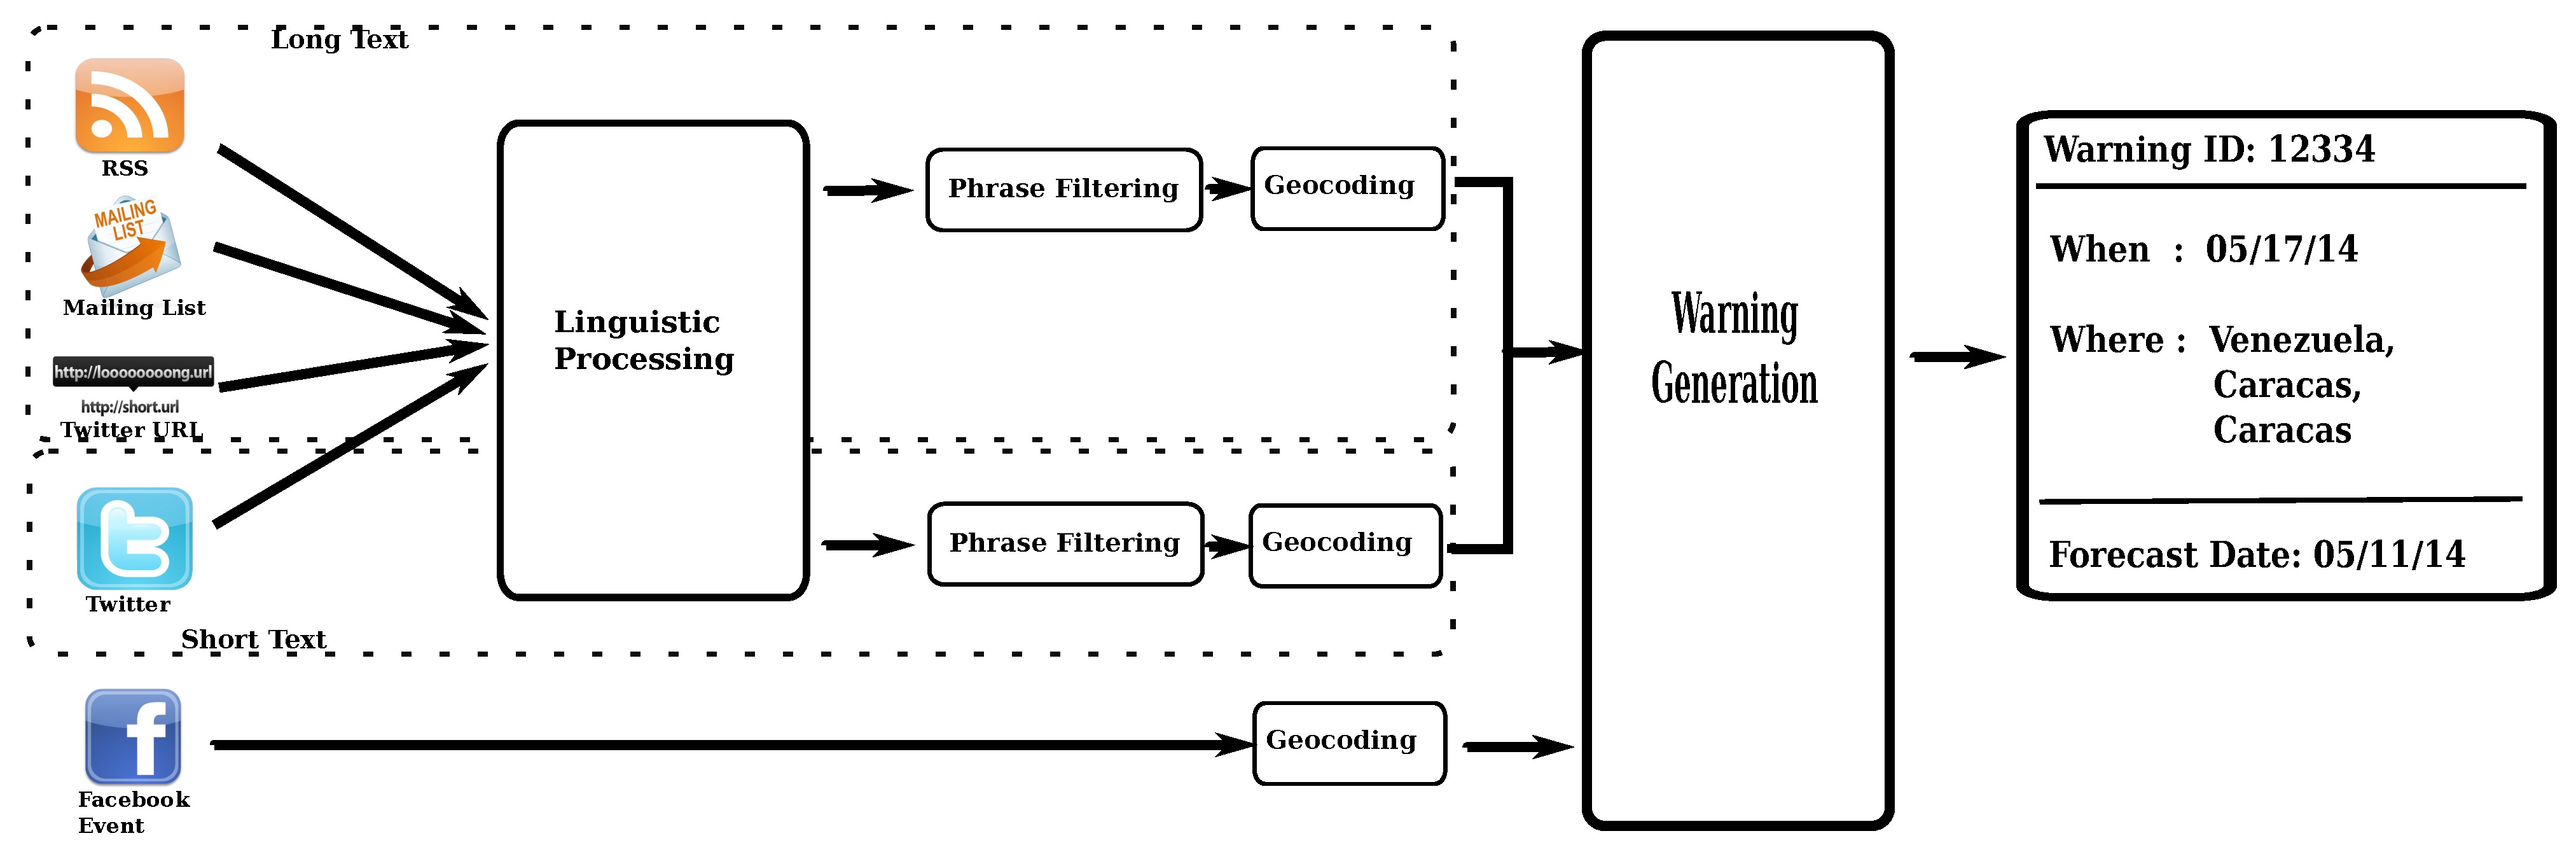
\includegraphics[height=0.6\textheight,width=\textwidth]{pipeline}
\end{figure}
\end{frame}

\begin{frame}
    \frametitle{Data Sources}
    \begin{itemize}
        \item
            Long Text
            \begin{itemize}
                \item
                    RSS Feeds
                    \begin{itemize}
                        \item
                            News
                        \item
                            Blogs
                    \end{itemize}
                \item
                    Twitter-URL
            \end{itemize}
        \item
            Short Text
                \begin{itemize}
                    \item
                        Twitter
                \end{itemize}
        \item
            Facebook-Event

    \end{itemize}
\end{frame}

\begin{frame}
    \frametitle{Long Text - RSS Feeds}
    \begin{itemize}
        \item
            Data Duration: November 2012 to March 2014
        \item
            6540 News
        \item
            6540 Blogs
        \item
            Talkwalker Alerts or Google Alerts
    \end{itemize}
\end{frame}

\begin{frame}
    \frametitle{Example - RSS Feed}
\end{frame}

\begin{frame}
    \frametitle{Short Text - Twitter}
    \begin{itemize}
        \item
            Datasift Firehose
        \item
            Duration November 2012 to March 2014
    \end{itemize}
\end{frame}

\begin{frame}
    \frametitle{Example}
\end{frame}

\begin{frame}
    \frametitle{Facebook}
    \begin{itemize}
        \item
            Facebook Graph API
        \item
            Facebook Query Language
    \end{itemize}
\end{frame}

\begin{frame}
    \frametitle{Example}
\end{frame}

\section{Preliminaries}
\begin{frame}
\frametitle{Preliminaries}
\end{frame}

\section{Linguistic Preprocessing}
\begin{frame}
    \frametitle{Natural Language Enrichment}
    \begin{itemize}
        \item
            Tokenization
        \item
            Lemmatization
        \item
            Noun Phrase Extraction
        \item
            Named Entity Extraction and Classification
    \end{itemize}
\end{frame}

\begin{frame}
\frametitle{TIMEN Enrichment}
    \begin{itemize}
        \item
            Extraction of Absolute Dates from text
        \item
            Identification of Relative dates like `yesterday, next wednesday' etc.
    \end{itemize}
\end{frame}

\section{Geocoding}
\begin{frame}
\frametitle{Geocoding- RSS Feeds}
\begin{figure}
    \centering
    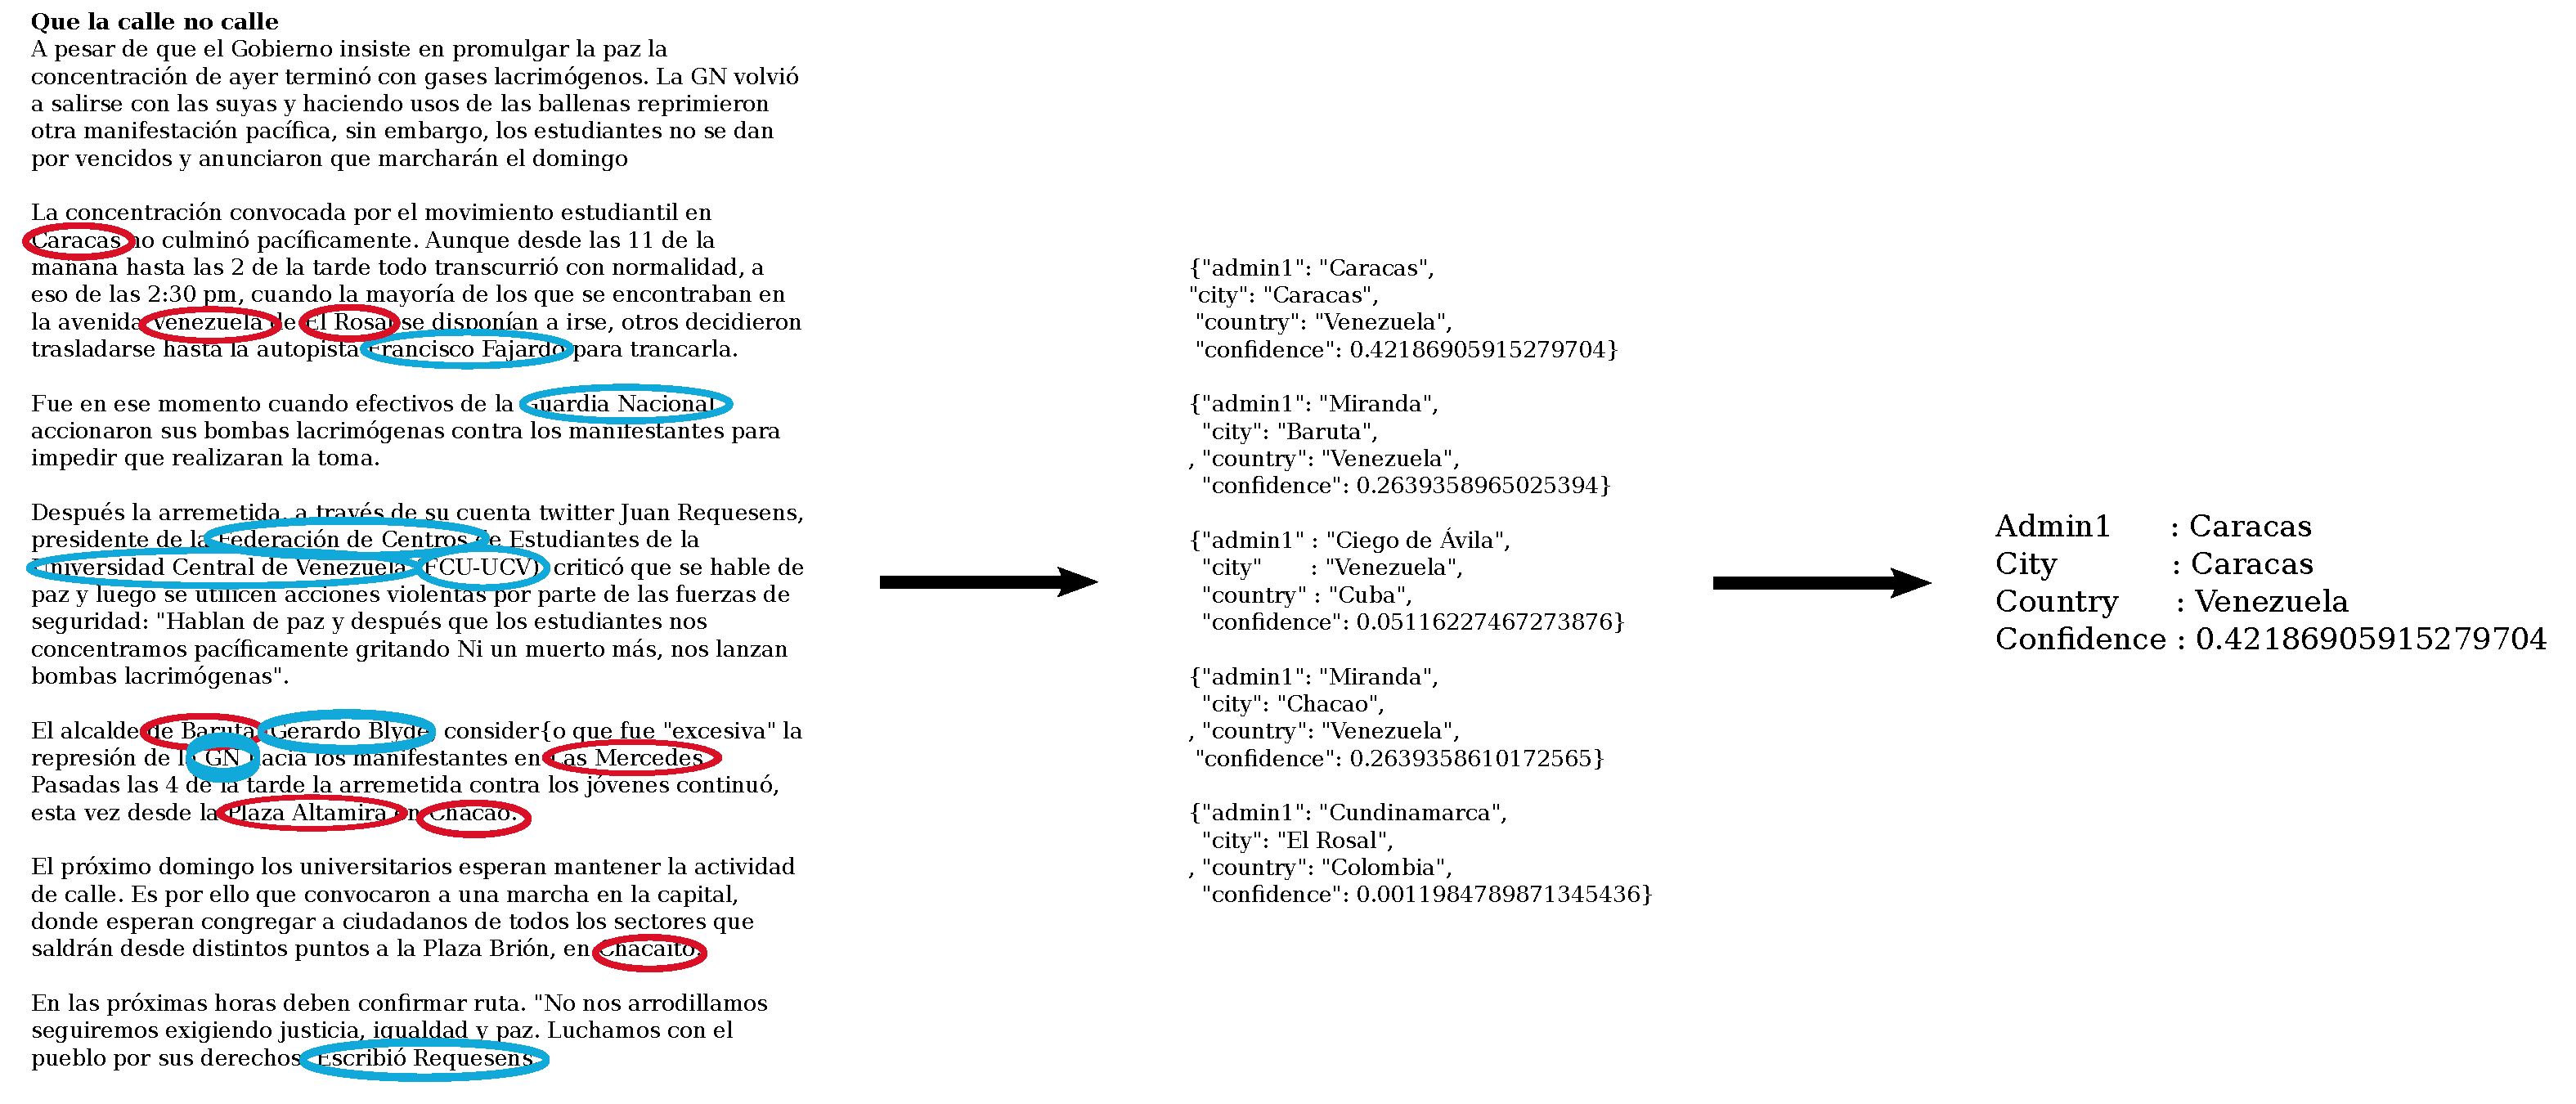
\includegraphics[width=\textwidth]{psl_pipeline2}
\end{figure}
\end{frame}

\begin{frame}
\frametitle{Geocoding- Twitter}
    \begin{itemize}
        \item
            Geotag of the tweet
        \item
            Twitter ``places" metadata
        \item
            Other text fields (user profile, tweet text)
    \end{itemize}
\end{frame}

\begin{frame}
\frametitle{Geocoding- Twitter}
    \begin{itemize}
        \item
            Facebook Location Objects
        \item
            Facebook Event Venue/location
    \end{itemize}
\end{frame}

\section{Phrase Matching}
\begin{frame}
\frametitle{Phrase Matching}
\end{frame}


\begin{frame}
\frametitle{Phrase List development}
\end{frame}


\begin{frame}
    \frametitle{Dependency Parsing}
\end{frame}


\begin{frame}
    \frametitle{Phrase List for Long Text}
\end{frame}


\begin{frame}
    \frametitle{Phrase List for Short text}
\end{frame}


\begin{frame}
    \frametitle{System Framework Once again}
\end{frame}

\begin{frame}
    \frametitle{Some Examples}
\end{frame}

\begin{frame}
     \frametitle{Venezuelan Spring}
     \begin{figure}
        \centering
        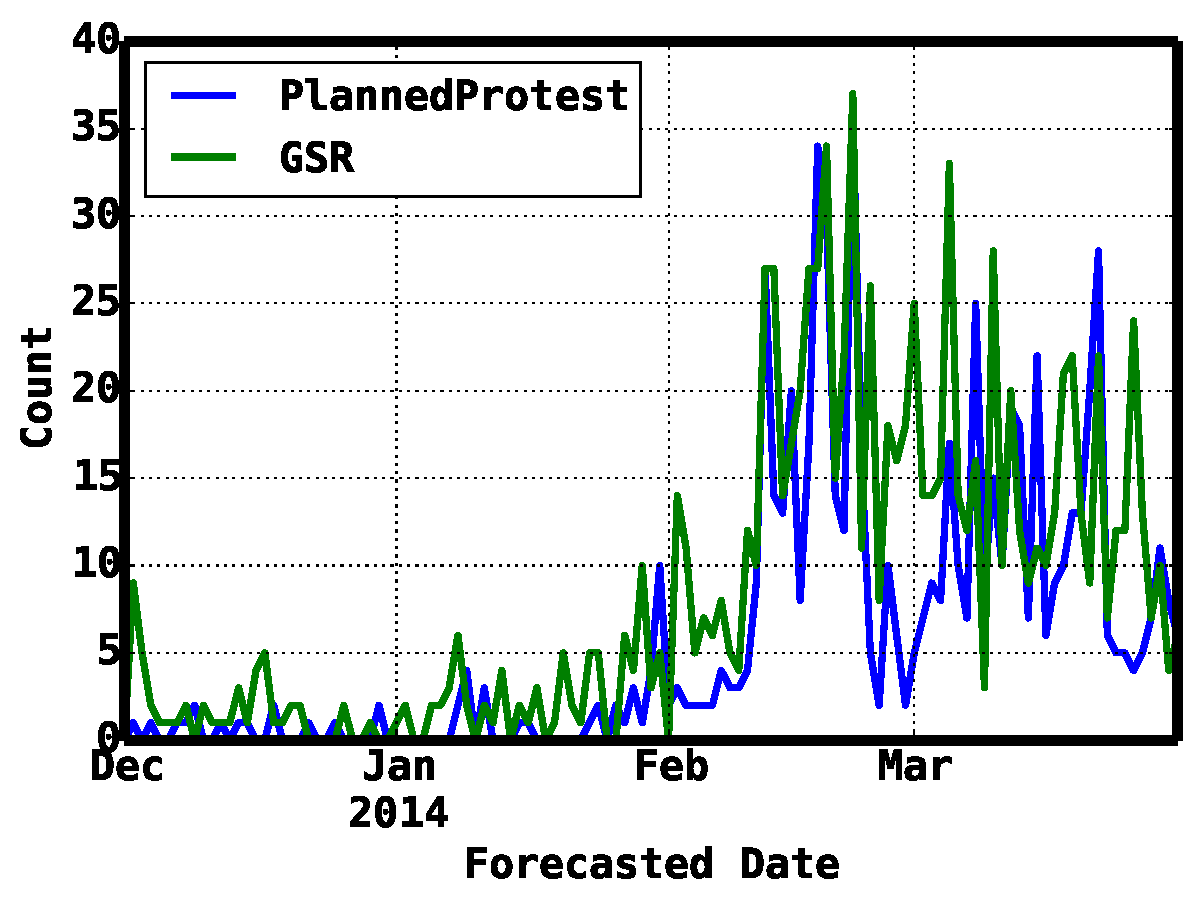
\includegraphics[width=\textwidth,height=0.8\textheight]{venezuela}
     \end{figure}
\end{frame}

\begin{frame}
    \frametitle{Venezuelan Violent Protests}
     \begin{figure}
        \centering
        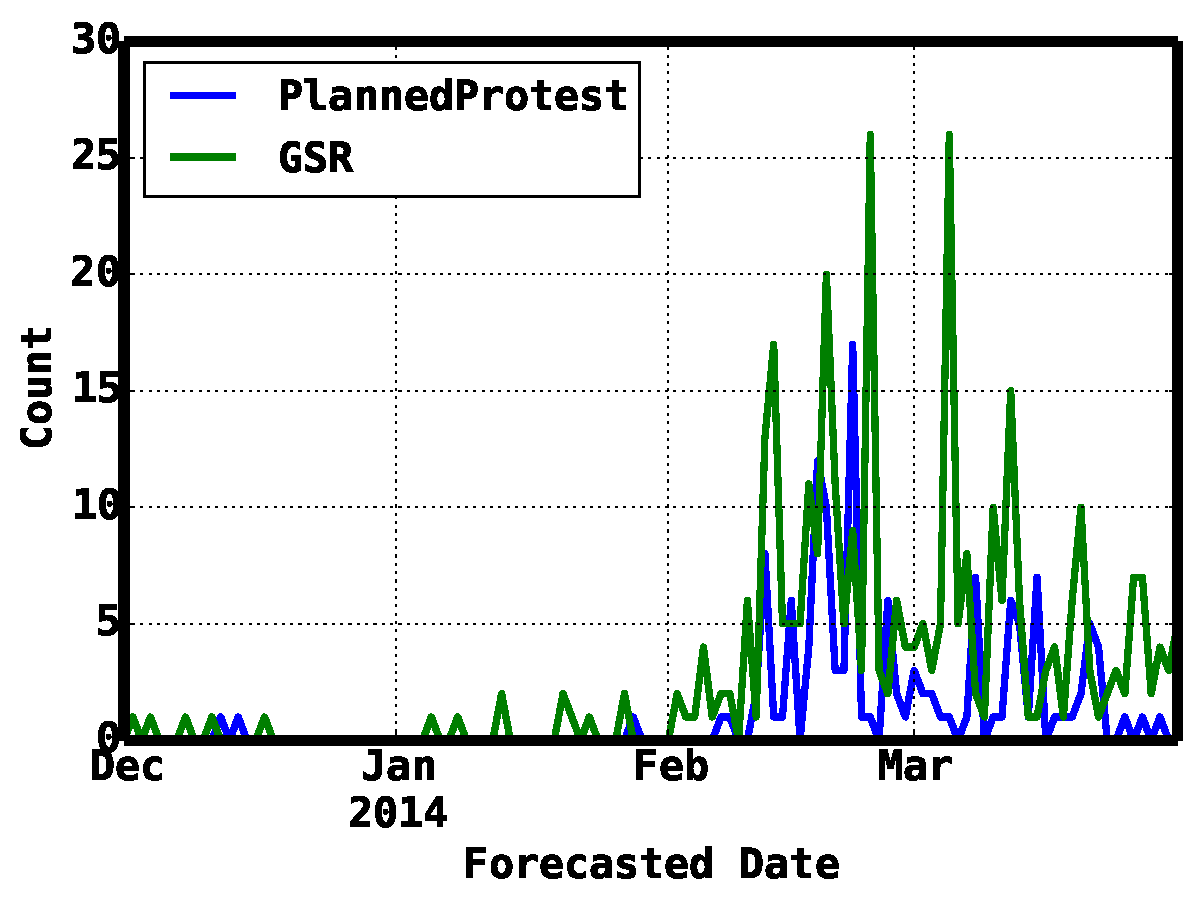
\includegraphics[width=\textwidth, height=0.8\textheight]{venezuela_violent}
     \end{figure}
\end{frame}

\begin{frame}
    \frametitle{Brazilian Spring}
    \begin{figure}
        \centering
        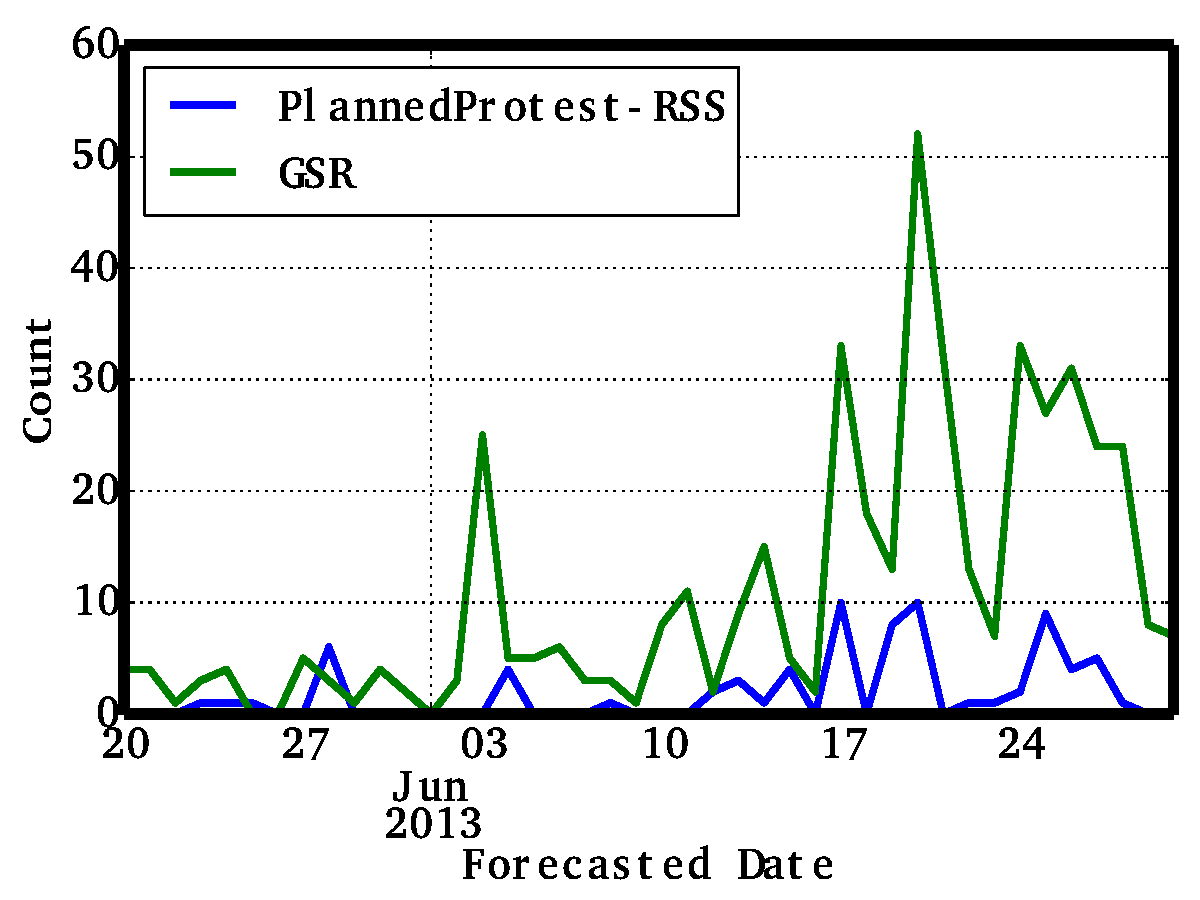
\includegraphics[width=\textwidth,height=0.8\textheight]{brazil_june}
    \end{figure}
\end{frame}

\begin{frame}
    \frametitle{Evaluation Methodology}
\end{frame}


\begin{frame}
    \frametitle{Goal Standard Report}
\end{frame}


\begin{frame}
    \frametitle{Comparison of Warnings against GSR}
\begin{figure}
\centering
\hfill
\subfigure[A]{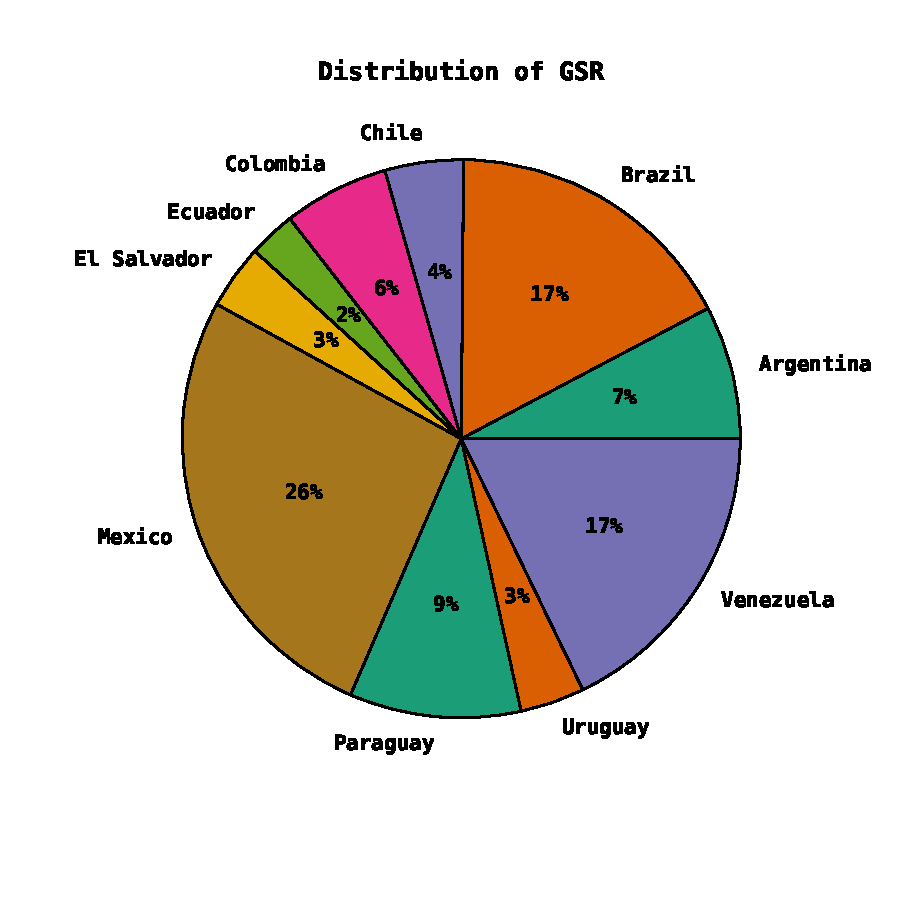
\includegraphics[width=0.5\textwidth]{gsr_distribution}}
\hfill
\subfigure[B]{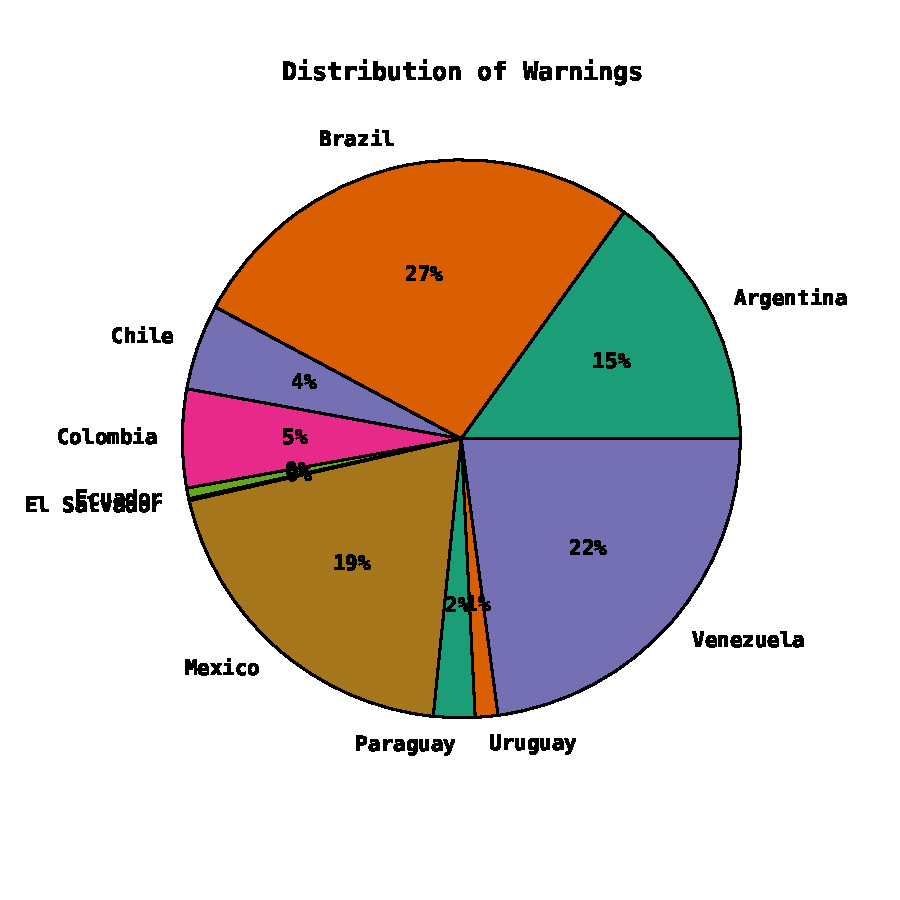
\includegraphics[width=0.5\textwidth]{pp_dist}}
\hfill
\caption{useless}
\end{figure}

\end{frame}


\begin{frame}
    \frametitle{Matching}
\end{frame}


\begin{frame}
    \frametitle{Individual Source Level Perfomance}
\end{frame}

\begin{frame}
    \frametitle{RSS Feeds + Twitter-Urls}
\end{frame}

\begin{frame}
    \frametitle{Twitter}
\end{frame}

\begin{frame}
    \frametitle{Facebook}
\end{frame}

\begin{frame}
    \frametitle{all Sources}
\end{frame}

\begin{frame}
    \frametitle{Quality Score over the months}
\end{frame}

\begin{frame}
    \frametitle{Quality Score with varying date thresholds }
\end{frame}

\begin{frame}
    \frametitle{Lead-Time vs Quality}
\end{frame}

\begin{frame}
    \frametitle{Quality Score Double Hump}
\end{frame}

\end{document}
